\section{问题建模}

\subsection{数据采集管线}

\subsubsection{Doppler雷达}

多普勒雷达感知的物理基础是多普勒效应。当雷达发射频率为$f_{c}$的连续波（CW）信号时，若目标相对于雷达存在径向运动，接收到的回波信号频率将发生偏移。

发射信号可表示为：

\begin{equation}
    s(t) = A\cos(2\pi f_{c}t + \phi_{0})
\end{equation}

其中 $A$ 为振幅，$\phi_{0}$ 为初始相位。当目标以速度 $v$ 运动时，回波信号的频率变化量（即多普勒频率 $f_{d}$）与径向速度的关系满足：

\begin{equation}
    f_{d} = \frac{2v}{\lambda}\cos\theta
\end{equation}

在此公式中，$\lambda$ 为电磁波波长，$\theta$ 为运动方向与雷达法线之间的夹角。对于手势识别而言，手掌的微小位移会引起回波相位的显著变化，这是实现高精度感知的核心。

当使用较低频率（如 5.8GHz）的雷达时，电磁波波长 $\lambda$ 与手掌的长宽 $L, W$ 处于同一数量级（即 $\lambda \approx L, W$）。在这种情况下，手掌既不能被视为点电荷（瑞利散射），也不能被视为无限大平面（几何光学散射），必须使用米氏理论来描述其散射特性。

在米氏散射区，目标的雷达散射截面积（RCS）对照射角度极其敏感。即便是同一个手势，只要手掌进入雷达波束的角度稍微改变几度，回波信号的幅度（Amplitude）和相位（Phase）分布就会发生剧烈波动，已有研究表明，多普勒频移不仅影响速度估计，还会与距离测量形成耦合关系，在高动态目标场景中容易造成距离估计偏移和滤波收敛变慢\cite{yu2026dopplerrange}。这种由米氏散射引起的"特征不稳定"是导致深度学习模型在不同用户间泛化性极差的根本原因。这里我们将幅度、相位等直接通过物理世界采集并做线性处理的变量称为"一阶特征"。

我们将手掌简化为一个具有确定性物理参数的导体矩形孔径。根据动态反射散射（DRS）理论，接收信号的复包络 $R(t)$ 可以表示为手掌表面所有散射点贡献的矢量和：

\begin{equation}
    R(t) = \int_{S}\sigma(s)e^{-j\frac{4\pi}{\lambda}d(s,t)}\, ds
\end{equation}

其中，$\sigma(s)$ 为散射系数，$d(s,t)$ 为随时间变化的传播距离。在近场（菲涅尔区）条件下，波前不能简化为平面波，必须考虑距离项的二阶近似，这导致了回波中存在非线性的相位调制特征。

由于多普勒回波是正弦调制的，直接观察时域波形难以提取线性运动特征。为了获取手势运动的真实轨迹，我们需要从正交信号（I/Q 信号）中解调出原始相位 $\Phi(t)$。

传统的解算方法在信号穿过坐标原点或信噪比（SNR）较低时易产生跳变。这里采用反正弦（arcsine）算法。该算法通过对归一化后的 I/Q 路信号进行反三角函数运算：

\begin{equation}
    \Phi(t) = \arcsin\left( \frac{I_{norm}(t)}{\sqrt{I_{norm}^{2}(t) + Q_{norm}^{2}(t)}} \right)
\end{equation}

该方法能够有效避免相位模糊（Phase Ambiguity），并将连续的手势动作转化为平滑的相位演化曲线。在米氏散射模型下，当手掌掠过雷达上方时，相位曲线会出现特征性的"极值点（Minima）"，这些极值点正是我们进行手势分类的确定性物理特征。

而为了获取手势的角度信息，我们使用时分复用单输入多输出架构（TDM-SIMO）通过周期性地切换发射或接收天线，在时域上形成虚拟的接收通道。

通过比较不同通道（天线单元）之间的相位差（AoA, Angle of Arrival），我们可以利用下式计算手势的空间角度：

\begin{equation}
    \Delta\Phi = \frac{2\pi d}{\lambda}\sin\theta
\end{equation}

其中 $d$ 为天线阵元间距。结合多普勒频率（速度维度）和相位差（角度维度），系统构建出了一个多维的特征向量空间，为后续基于 SVM 或轻量化 MLP 的分类器提供了高辨识度的数据输入。

\subsubsection{雷达信号处理}

本研究采用基于 MAX2829 的多通道射频前端电路，构建了一个高度相干的 TDM-SIMO 雷达系统。为了满足手势识别对微多普勒相位（Micro-Doppler Phase）的高精度要求，系统在硬件设计上采用了同源时钟方案。由晶振（XTAL）产生的参考信号经 CDCLVC1104 时钟缓冲器一分为四，同步供给发射端、接收端以及 STM32F103 主控模块。这种时钟分配策略确保了下变频过程中本振信号与发射信号的相位一致性，为后续提取具有物理意义的确定性多普勒相位\cite{lien2016soli}奠定了相干性基础。

\begin{figure}[htbp]
    \centering
    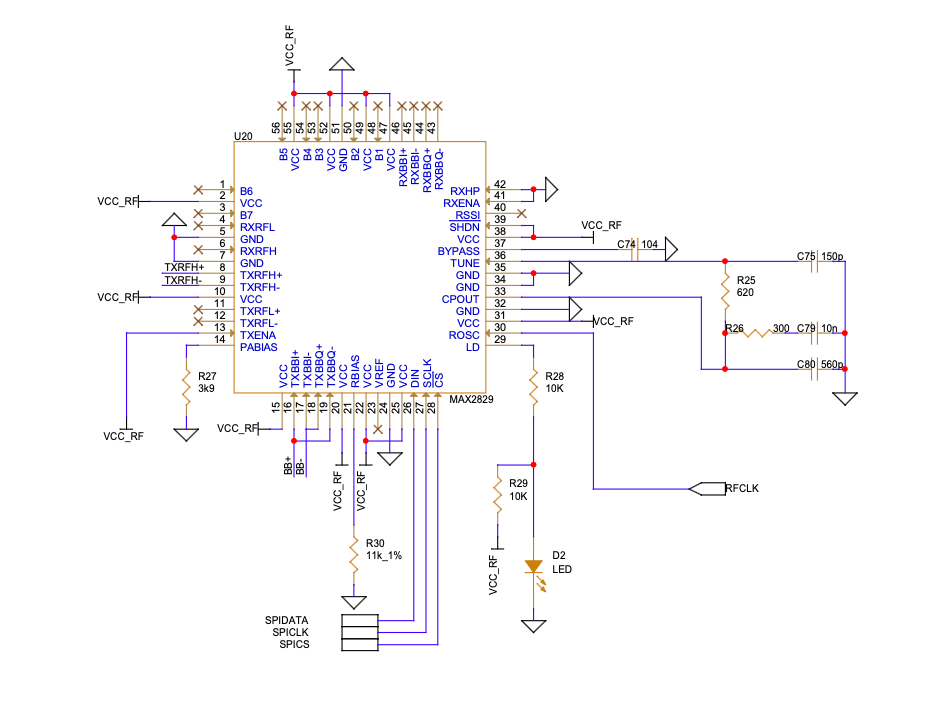
\includegraphics[width=0.9\textwidth]{doc_thesis/figs/04/max2829_schematic.png}
    \caption{\ptheadingfont{MAX2829电路原理图}}
    \label{fig:max2829}
\end{figure}

在信号流向上，接收天线捕捉到的微弱回波经 HMC7992 射频开关切换进入 SKY65404 低噪声放大器，随后在 MAX2829 片内完成下变频处理。输出的差分 I/Q 基带信号通过 INA2331 仪表放大器转换为单端信号，并利用 PFS455A 低通滤波器执行抗混叠滤波，最终由 MCU 的内置 ADC 进行数字化采样。

\begin{figure}[htbp]
    \centering
    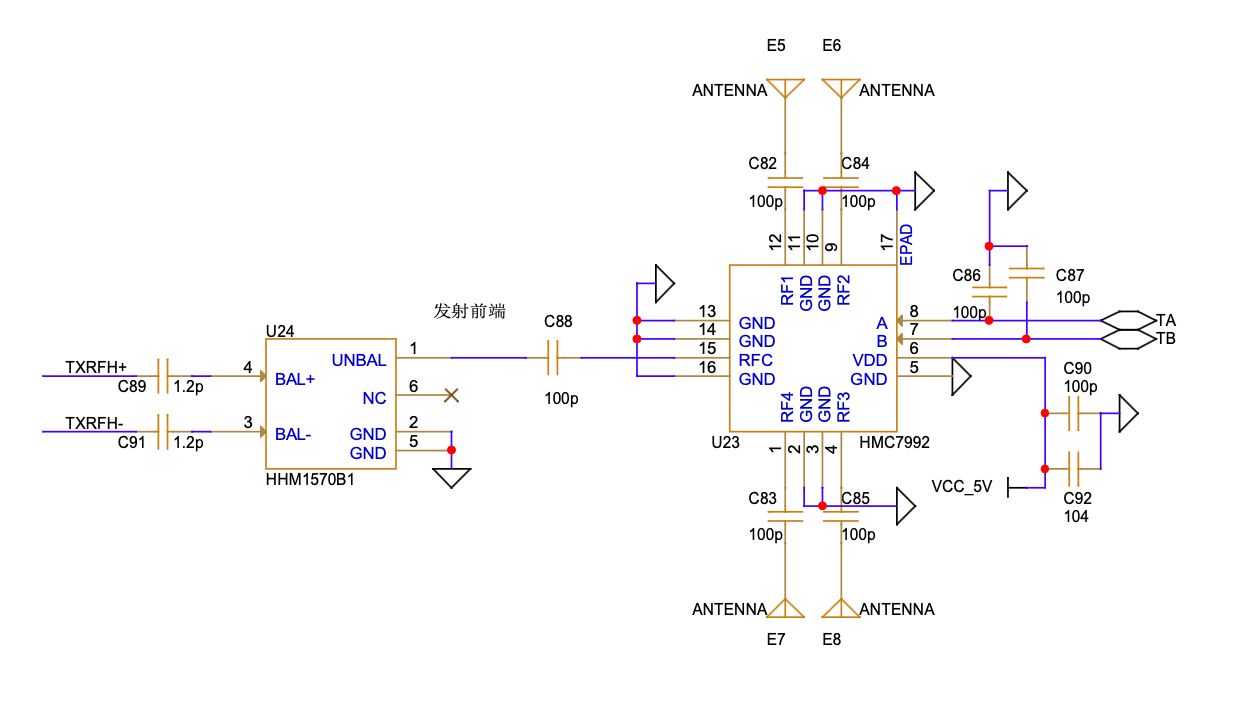
\includegraphics[width=0.85\textwidth]{doc_thesis/figs/04/hmc7992_schematic.png}
    \caption{\ptheadingfont{HMC7992电路原理图}}
    \label{fig:hmc7992}
\end{figure}

为了从数字化后的 I/Q 序列中准确解算出手势动态特征，本系统遵循了以下的处理流程：针对 TDM 采样带来的通道间时间异步，利用数字相位移动滤波器进行时域补偿，并采用梯度下降算法消除硬件引入的直流偏置（DC Offset）；采用反正弦（arcsine）算法线性重构多普勒相位 $\Phi(t)$。该算法通过计算相邻采样点间的 I/Q 交叉乘积，有效抑制了手掌在米氏散射区（Mie Region）因照射角度变化产生的幅度震荡（Amplitude Variation），从而提取出与目标位移直接挂钩的相位信息。

\subsection{确定性信号与神经网络分类}

\subsubsection{手势信号采集物理建模}

对于第 $i$ 个 TDM 接收通道，其数字基带 I/Q 信号可建模为

\begin{equation}
    I_{i}[n] = A_{I,i}[n]\cos(\Phi_{i}[n]) + dc_{I,i} + n_{I,i}[n]
\end{equation}

\begin{equation}
    Q_{i}[n] = A_{Q,i}[n]\sin(\Phi_{i}[n]) + dc_{Q,i} + n_{Q,i}[n]
\end{equation}

其中 $A_{I,i}[n]$，$A_{Q,i}[n]$ 表示随时间缓慢变化的幅度项，$dc_{I,i}$，$dc_{Q,i}$ 为直流偏置，$n_{I,i}[n]$，$n_{Q,i}[n]$ 为噪声项，而 $\Phi_{i}[n]$ 为多普勒相位。

对于电磁波而言，检测物体距离电磁波发射源的距离会直接体现在多普勒信号的相位上：

\begin{equation}
    \Phi_{i}[n] = \Phi_{i}[0] + \sum_{j=1}^{n}\Delta\Phi_{i}[j]
\end{equation}

为了从 $I/Q$ 信号中稳定地提取相位增量 $\Delta\Phi_{i}[j]$，并抑制幅度波动的影响，采用反正弦（arcsine）解调算法，其表达式为

\begin{equation}
    \Delta\Phi_{i}[j] = \arcsin\frac{I_{i}[j]Q_{i}[j+1] - I_{i}[j+1]Q_{i}[j]}{\sqrt{I_{i}^{2}[j+1] + Q_{i}^{2}[j+1]}\sqrt{I_{i}^{2}[j] + Q_{i}^{2}[j]}}
\end{equation}

该公式利用归一化后的 I/Q 正交关系，使提取的结果主要反映相位变化而非幅度变化，从而得到与目标运动高度相关的相位序列。

上述得到的多普勒相位变化本质上来源于检测物体到雷达天线的物理距离变化。建立三维笛卡尔坐标系，假设物体坐标 $(x_{t}, y_{t}, z_{t})$

\begin{equation}
    \left\{ \begin{aligned}
    L_{1} &= \sqrt{(x_{t}+a)^{2}+(y_{t}-a)^{2}+z_{t}^{2}} + \sqrt{(x_{t}-a)^{2}+(y_{t}-a)^{2}+z_{t}^{2}} \\
    L_{2} &= \sqrt{(x_{t}+a)^{2}+(y_{t}-a)^{2}+z_{t}^{2}} + \sqrt{(x_{t}-a)^{2}+(y_{t}+a)^{2}+z_{t}^{2}} \\
    L_{3} &= \sqrt{(x_{t}+a)^{2}+(y_{t}-a)^{2}+z_{t}^{2}} + \sqrt{(x_{t}+a)^{2}+(y_{t}+a)^{2}+z_{t}^{2}}
    \end{aligned} \right.
\end{equation}

其中，$L_{1}, L_{2}, L_{3}$ 代表信号从发射端到手势目标再到三个接收端的完整空间往返路径长度；$(x_{t}, y_{t}, z_{t})$ 代表手势散射相位中心的瞬时三维空间坐标；$a$ 代表天线阵列分布的固定几何常数（即原点到天线的投影距离）。

在多收单发（SIMO）的双基地雷达空间架构中，手势目标的三维运动会导致空间电磁波传播路径的动态变化。目标产生的瞬时多普勒角频率不仅取决于其绝对速度，更取决于速度向量在发射与接收路径上的空间投影。其核心运动学映射关系可表示为：

\begin{equation}
    \omega_{d,i}(t) = \frac{d\Phi_{i}(t)}{dt} = -\frac{2\pi}{\lambda}\left(\vec{v}(t) \cdot \hat{u}_{T}(t) + \vec{v}(t) \cdot \hat{u}_{R,i}(t)\right)
\end{equation}

其中，$\omega_{d,i}(t)$ 代表第 $i$ 个接收通道提取出的瞬时多普勒角频率；$\lambda$ 为雷达发射信号的载波波长；$\vec{v}(t)$ 为手势目标在三维空间中的瞬时速度矢量；$\hat{u}_{T}(t)$ 与 $\hat{u}_{R,i}(t)$ 分别代表从手势散射中心指向发射天线和第 $i$ 个接收天线的单位方向向量。

由于天线阵列在空间上的分布式二维布局，特定轨迹的手势（如"向右滑动"）在经过检测区域时，其到达各个接收天线的距离变化率存在确定的先后顺序。这种物理层面的空间几何差异，经过上述算法解调后，直观地表现为三路接收信号相位极小值 $-\Phi_{i}(t)$ 出现的时间差。该时序特征规律具有高度的确定性，且对目标所处高度 $h$ 具有良好的鲁棒性，从而构成了手势分类识别的核心特征依据。

\subsubsection{确定性信号建模}

根据前文推导的电磁散射模型，当手掌运动的角度或形态发生微小变化时，接收到的 I/Q 回波幅度会发生剧烈的非线性震荡，导致传统谱图特征（基于FFT或STFT生成的幅度包络）极易失效。然而，尽管幅度受到严重干扰，信号的相位演化却遵循明确的物理几何约束。通过引入近场条件下的二阶距离近似，我们将单向手势运动产生的时变相位轨迹 $\Phi_{i}(n)$ 建模为一个受几何拓扑主导的凸函数。本文的"确定性"正是建立在这一物理现象之上：即无论动作的快慢、手掌的大小，甚至是因散射造成的轻微幅度失真，只要手势的拓扑轨迹（如"左滑"、"右滑"）不变，其在不同接收通道产生相位曲线 $-\Phi_{i}(n)$ 的极小值（Minima）的相对时间顺序（Temporal Sequential Order）是确定的、不受干扰的常量\cite{lien2016soli}。

为了从含有噪声的基带信号中"提纯"这一确定性特征，系统设计了一条严密的数字信号处理（DSP）管线：首先，针对TDM-SIMO架构造成的通道间时间异步，系统利用全通相移滤波器进行对齐，得到包含完整物理意义的 $(T, 6)$ 维 I/Q 矩阵。随后，为抑制幅度波动，引入反正弦（arcsine）算法解算出相位增量并累加得到多普勒相位。

在信号分割环节，我们避开了复杂的神经网络检测，转而计算差分功率 $\Delta P[n]$，由于微小手势和静态杂波引起的相位跳变存在量级差异，通过设立随环境自适应的阈值，将连续回波裁剪为包含单一动作的最宽运动段 $[n_{a}, n_{b}]$。

最后，为消除动作执行速度带来的时间维度变异，我们将该区间归一化至 $[0, 1]$，并通过八阶多项式拟合剔除高频相位抖动。对于平滑后的 $\Phi_{i}(t)$ 曲线，系统提取各通道的最小值时刻 $t_{m,i}$，从而将原始的 $(L, 3)$ 维度的相位数据，简化为确定性的三维特征向量 $\boldsymbol{t}_{m} = (t_{m,1}, t_{m,2}, t_{m,3})$。

这一基于物理引导的特征提取方案，从根本上改变了后续分类网络的工作负载。传统的 DCNN 或 RNN 网络需要处理数十万参数来拟合庞大且复杂的时频谱图特征矩阵，这不仅消耗大量内存，还需要海量的训练数据来防止过拟合。

与之形成鲜明对比的是，将手势识别从高维的"图像分类"问题，降维成了明确的"三维空间点聚类"问题。这种极简的确定性特征不仅对由于体型差异和操作距离造成的散射变异具有天然免疫力，而且仅需部署如 SVM（如 OVR-SVM 架构）或轻量级的全连接网络（MLP）即可实现极高的分类准确率。这一"白盒化"的建模思路，极大地降低了端侧设备的推理延迟，使雷达手势识别在低功耗智能终端上的实时部署成为可能。

对于确定性信号方法假设每个手势样本前后都有明确的静止段（quiet period），我们测试记录按下空格键到松开空格键之间的纯动作段，不包含动作前后的静止区间。直接用原论文方法处理这些数据，确定性信号方法准确率仅约 15\%（接近随机）。

然而当我们能够获取整个流程的手势动作的时候，包括手势之间的自然静止间隔（约 280个采样点，更加贴合常规场景下人类的使用逻辑），我们通过互相关匹配将每个手势片段定位回连续信号流中的精确位置，然后向前后各扩展一段采样窗口，提取出真实的静止区域信号。仅利用扩展得到的静止区域估计各通道的直流分量，再从整段信号中减去。我们改用信号功率（$I^2 + Q^2$）的峰值时间作为时间特征，通过高阶多项式拟合定位峰值。功率峰值反映手势运动最剧烈的时刻，对起止边界的精确性要求更低，鲁棒性显著优于相位最小值法。这避免了用手势动态信号参与DC估计所带来的偏差，这种方法的优势便在于：不要求用户在动作前后刻意停留，而是利用连续采集的原始信号流自动回溯手势间自然存在的静止间隔，恢复确定性信号方法所需的参考基线；同时将时间特征从对边界敏感的相位最小值改为对边界鲁棒的功率峰值，从而在不牺牲交互自然性的前提下实现高精度分类。

\subsubsection{网络层级和结构}

本研究涉及的手势识别在数据形态上分为两类：一是对齐后的多通道 I/Q 随时间采样，可建模为变长序列；二是经前端处理得到的低维确定性特征向量（如各接收通道相位曲线上的标量特征），适合作为静态向量输入。对应地，可采用序列模型刻画时序依赖，或采用基于核的分类器在紧凑特征空间中线性/非线性可分；若另有多视角或成像式表征，还可采用卷积网络迁移学习。

简单网络中的支持向量机（Support Vector Machine, SVM）是一种基于统计学习理论中结构风险最小化原则的监督学习算法，其核心目标是在高维特征空间中寻找一个能够实现类间跨度最大化的最优决策超平面。对于给定数据集 $D = \{(x_{i}, y_{i})\}_{i=1}^{n}$，其中 $x_{i} \in \mathbb{R}^{d}$ 为特征向量，$y_{i} \in \{-1, 1\}$ 为类别标签，SVM 试图构建线性方程 $w^{T}x + b = 0$ 确定的划分超平面，其中 $w$ 为决定超平面方向的法向量，$b$ 为偏置项。为了增强模型的泛化能力，SVM 要求最小化 $\|w\|^{2}$ 以实现几何间隔 $2/\|w\|$ 的最大化，由此转化为一个带约束的凸二次规划问题：$\min_{w,b}\frac{1}{2}\|w\|^{2}$ 满足 $y_{i}(w^{T}x_{i} + b) \geq 1$。在实际应用中，考虑到数据噪声引起的线性不可分问题，模型引入松弛变量 $\xi_{i}$ 和惩罚参数 $C$ 构造软间隔（Soft Margin）目标函数，即 $\min_{w,b,\xi}\frac{1}{2}\|w\|^{2} + C\sum_{i=1}^{n}\xi_{i}$，通过调节 $C$ 在间隔最大化与误分类容忍度之间取得平衡。针对复杂的非线性映射需求，SVM 通过拉格朗日对偶性（Lagrangian Duality）将原始问题转化为对偶形式，并利用核技巧（Kernel Trick）引入核函数 $K(x_{i}, x_{j})$。该技术通过将低维空间的输入映射至高维再生核希尔伯特空间（Reproducing Kernel Hilbert Space, RKHS），使得原本线性不可分的数据在高维空间中变得线性可分，从而在不显式增加计算复杂度的情况下处理高度非线性的分类任务。

还可以通过传统神经网络中的CNN/DNN网络进行分析，得到六通道雷达信号后，对时域的连续波进行频域变换得到全彩多普勒频谱图（PDS, Panchromatic Doppler Spectrograms），从离散时域 I/Q 信号生成这些图像

\begin{equation}
    \mathrm{STFT}_{i}[m,k] = \sum_{n=0}^{N_{w}-1}\varphi_{i}[n + m \cdot H] \cdot w[n] \cdot e^{-j2\pi kn/N_{w}}
\end{equation}

其中 $w[n]$ 为Hanning 窗函数，窗长 $N_{w} = 20$：

\begin{equation}
    w[n] = \frac{1}{2}\left(1 - \cos\left(\frac{2\pi n}{N_{w}-1}\right)\right), \quad n = 0, 1, \ldots, N_{w}-1
\end{equation}

$H = 10$ 为跳步长度（hop size），即 50\% 重叠（overlapping points $= N_{w} - H = 10$），$m$ 为时间帧索引，$k$ 为频率 bin 索引。每通道得到的谱图强度（功率谱密度）为

\begin{equation}
    S_{i}[m,k] = |\mathrm{STFT}_{i}[m,k]|^{2}
\end{equation}

结果是一张二维单色谱图（时间帧 $\times$ 频率 bin），如图~\ref{fig:spectrogram_3ch}所示：

\begin{figure}[htbp]
    \centering
    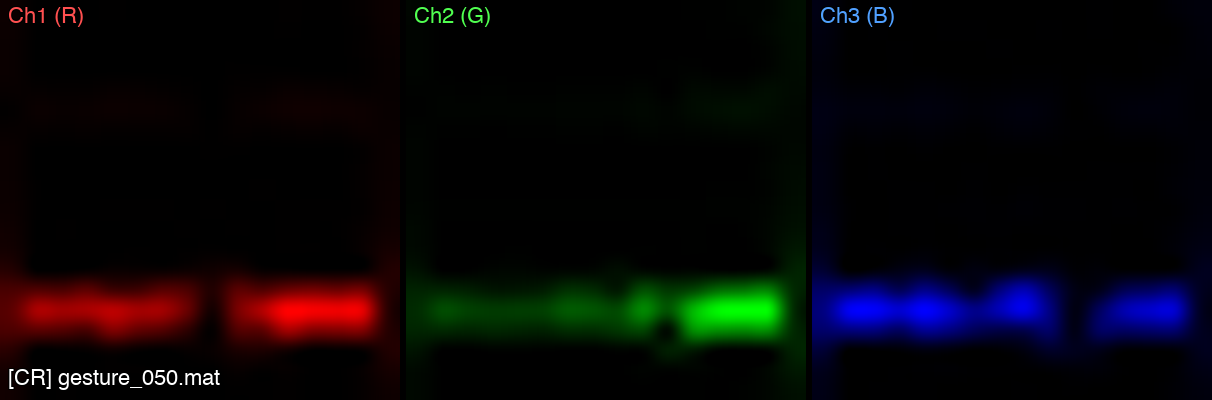
\includegraphics[width=0.9\textwidth]{doc_thesis/figs/04/spectrogram_3ch.png}
    \caption{\ptheadingfont{单通道频谱图}}
    \label{fig:spectrogram_3ch}
\end{figure}

将每张谱图的强度归一化到 $[0, 1]$：

\begin{equation}
    \hat{S}_{i}[m,k] = \frac{S_{i}[m,k]}{\max_{m',k'}S_{i}[m',k']}
\end{equation}

然后将所有谱图统一缩放（resize）到 $400\times400$ 像素。再将三路天线的归一化谱图分别映射到 RGB 三个颜色通道，合成一张全彩图像：

\begin{equation}
    \mathrm{Image}[m,k] = \left(\hat{S}_{1}[m,k],\ \hat{S}_{2}[m,k],\ \hat{S}_{3}[m,k]\right) \in [0,1]^{3}
\end{equation}

因此我们就将时序信号识别的问题转化成了对RGB三通道像素数据的识别，由于各个动作的全彩PDS的类间差别较大，经过CNN/DNN特征提取后的特征分布应呈现明显的聚类效果，因此各个动作数据集规模并不庞大，相反地，如果动作的类间相似度非常高，就需要更多的数据集和边缘样本。即便在当前数据集并不庞大的情况下，其所需要的计算和空间存储成本远高于简单支持向量机SVM或多层感知机MLP的。

循环神经网络\cite{williams1989rnn}（RNN）和基于RNN改进的长短期记忆递归神经网络\cite{hochreiter1997lstm}（LSTM）是另一种解决方案：完全端到端（End-to-End），不做任何显式特征提取，让网络直接从原始波形中学习。优势在于流程最简、对先验知识的依赖最小；代价是模型作为黑盒缺乏可解释性，且在小样本场景下性能可能不如物理驱动的特征方案。并且由于时序模型每次处理的基本单位为帧窗口，计算速度天然相比于基于单帧全彩图片的CNN更加缓慢，也需要更大的存储空间和计算开销。

相比较于传统的高维数据序列分析得到频谱特征，使用CNN对频谱特征进行分析和训练；以及直接使用RNN/LSTM对时序进行分析训练，这种方法极大程度减少了训练端侧所需的时间和推理端侧所需要的算力成本。

\begin{table}[htbp]
    \centering
    \caption{\ptheadingfont{三种分类方法对比}}
    \label{tab:method_compare}
    {\zihao{5}\setlength{\extrarowheight}{2pt}%
    \begin{tabularx}{\linewidth}{|>{\centering\arraybackslash}p{2.2cm}|>{\centering\arraybackslash}X|>{\centering\arraybackslash}X|>{\centering\arraybackslash}X|}
        \hline
         & \textbf{支持向量机（SVM）} & \textbf{卷积神经网络（CNN）} & \textbf{带有时序的网络（RNN/LSTM）} \\
        \hline
        输入 & $t_{m} \in \mathbb{R}^{3}$ & $x \in \mathbb{R}^{C \times H \times W}$ & $t \in \mathbb{R}^{6 \times T}$ \\
        \hline
        训练数据量 & 很少（十个样本以内即可收敛） & 较多（数十张图片） & 较多 \\
        \hline
        训练时间 & 最短（$<$5s） & 较长（$<$10min） & 中等 \\
        \hline
        占用空间 & 小\newline（可在CPU运行） & 中\newline（Apple 654.7MB\newline $\approx$ cuda 1.0--1.2GB） & 小\newline（Apple 54.4MB\newline $\approx$ cuda 0.4--0.6GB） \\
        \hline
    \end{tabularx}}
\end{table}

\section{实验设计}

\subsection{硬件电路}

整个实验平台由射频（RF）板卡和上位机两部分组成。

\begin{table}[htbp]
    \centering
    \caption{\ptheadingfont{射频硬件平台设计}}
    \label{tab:hardware}
    {\zihao{5}\setlength{\extrarowheight}{2pt}%
    \begin{tabularx}{\linewidth}{|>{\centering\arraybackslash}p{2.5cm}|>{\centering\arraybackslash}X|>{\centering\arraybackslash}X|}
        \hline
        \textbf{组件} & \textbf{型号/规格} & \textbf{功能} \\
        \hline
        微控制器 & STM32F103T8U6 & 系统控制、ADC 采样、数据传输 \\
        \hline
        射频收发芯片 & Maxim MAX2829 $\times$ 2 & 一片发射、一片接收，工作在 5.8 GHz \\
        \hline
        射频开关 & HMC7992 & 时分复用切换 3 路接收天线 \\
        \hline
        天线 & 倒 F 天线 $\times$ 4（1 发 3 收） & $y$ 方向极化，L 形排列 \\
        \hline
        USB-UART 桥接 & Silicon Labs CP2102 & 将采样数据传至上位机 \\
        \hline
        供电 & 标准锂电池 & 通过 SMP 同轴连接器供电 \\
        \hline
        连接方式 & 4 路 SMP 同轴连接器 & 天线板与 RF 板之间 \\
        \hline
    \end{tabularx}}
\end{table}

天线按 L 形排列在约 $5\,\text{cm} \times 5\,\text{cm}$ 的正方形区域内，平放于桌面，射频参数配置具体为：载波频率通过 MAX2829 的寄存器 3/4/5 配置为约 5.8 GHz；发射增益固定（寄存器 12 = 0x0034）；接收增益基准 RXp = 0x002F，三路天线分别设置为 RXp-3、RXp-4 和 RXp 以补偿各路径的增益差异。上电后需等待约 1 秒让 MAX2829 内部锁相环完成锁定。

采样系统方面，STM32 的 ADC1 和 ADC2 工作在双路同步模式，ADC1 采集 I（同相）分量，ADC2 采集 Q（正交）分量，由 TIM3 的 TRGO 信号触发以保证等间隔采样。DMA 自动将 ADC1 的 32 位数据寄存器搬运到内存变量 q[0]，其中高 16 位为 Q 分量、低 16 位为 I 分量。TIM3 配置为 ARR = 95、PSC = 999，在60 MHz 系统时钟下单次中断周期为1.6ms。每 5 次中断可以构成一个完整的 TDM 周期（依次采集 3 路天线和 1 路参考通道，第 5 次中断负责输出数据），因此有效输出速率为 $1/(5\times1.6) = 125\,\text{Hz}$。每行串口输出包含 6 个十进制整数 Q1 I1 Q2 I2 Q3 I3，分别对应三路接收天线在该 TDM 周期内的 I/Q 采样值，取值范围 0--4095（12 位 ADC）。

\subsection{手势定义和数据采集规范}

以雷达板所在平面为参考，定义坐标系为 $+x$ 向右、$+y$ 向前（远离操作者）、$+z$ 向上。总共定义 9 类手势，对应智能设备多点触屏的常见交互操作。其中 5 类为基本手势：L（向左横扫 $-x$ 方向，对应屏幕左翻页）、R（向右横扫，$+x$ 方向，对应右翻页）、F（向前推出，$+y$ 方向，对应屏幕上滚）、B（向后拉回，$-y$ 方向，对应屏幕下滚）、TAP（垂直方向按下再抬起，$\pm z$ 方向，对应点击）。另外 4 类对角线手势为冗余手势：LF（左前）、LB（左后）、RF（右前）、RB（右后），它们被定义为无效动作——当分类器识别出对角方向运动时，将其判定为无效输入而非误分类为某个基本手势。

对于开题报告中提到的细微化操作和任务，我们着重探究三种方法中哪一种的适用性最强，同时鉴于波长的物理约束，我们采用以下精密手势：手势的旋转：AR（逆时针旋转，手掌摊平，平行于天线平面，逆时针转动手腕180度）、CR（顺时针旋转，手掌摊平，平行于天线平面，顺时针转动手腕180度），这为前面的平动增加了手势转动的维度。

在数据采集时将雷达板平放于桌面、天线面朝上，操作者坐或站在板卡正前方，确保采集区域上方无其他运动物体。执行横扫类手势时，手掌底部距天线平面高度约 10 cm，横向行程约 9 cm（覆盖天线区域），全程保持平滑匀速；执行 TAP 手势时，手掌最近距离不小于 5 cm。匀速运动是保证多普勒相位为确定性曲线的关键前提。

单次采集的节奏为：静止约 1 秒 $\rightarrow$ 执行手势约 0.5--1 秒 $\rightarrow$ 静止约 1 秒 $\rightarrow$ 下一次。相邻手势之间的静止间隔使得差分功率分段算法能够通过信号能量的突变自动识别手势的起止边界。每次手势持续 0.5--1 秒，对应串口输出约 60--125 行数据（125 Hz 采样率）。系统在采集期间持续不间断输出，需要手动或通过标注文件记录每个手势对应的起止行号。

同时我们会发现所采集的信号必须符合一定的特定范式（静止-移动-静止），这些动作高度依赖静止-移动、移动-静止的状态变换。

采集的串口数据经 MATLAB 解析后存储为".mat"文件，每个文件包含一个名为 dat 的 $3 \times T$ 复数矩阵（complex double），3 行对应 3 路接收天线，实部为 I 分量、虚部为 Q 分量，时间长度 $T$ 随手势持续时间变化。

\subsection{数据集与训练参数}

我们采集总共约570个样本，每个类别样本约50～60个，采用5折（5 fold）训练法增强训练鲁棒性，即将数据集随机均等划分为5份，每次训练选择其中4份作为训练集，1份作为测试集，纵向评估5个训练的训练效果，选取效果最好的一份。

采集的原始数据在进入分类流水线之前需经过质量筛选，首先检查每条天线的负相位曲线，在手势段内是否只有恰好一个极小值，多个极小值意味着手势执行不规范（如中途停顿或速度不均匀），应予以丢弃，其次确认三个通道在手势期间均有明显的 I/Q 幅度变化，排除因天线遮挡或信号丢失导致的无效样本。最后检查极小值的时序是否符合对角手势的特征模式，若符合则标记为无效手势。此外，手势前后的静止间隔不足会导致差分功率分段算法无法正确提取手势区间，此类样本也需要剔除。

在 $k$ 分类任务中，假设总样本数量为 $N$，实验指标如下：准确率Acc（Accuracy）表示模型在所有类别中正确判断的样本数占总样本数的比例，反映了模型的整体分类性能，其中 $TP_{i}$ 为第 $i$ 类被正确预测为第 $i$ 类的样本数：

\begin{equation}
    \mathrm{Accuracy} = \frac{\sum_{i=1}^{k}TP_{i}}{N}
\end{equation}

精确率Prec（Precision）衡量模型"查准"的能力。对于多分类任务，通常采用 Macro-Precision（宏精确率），即先计算每个类别的精确率（正确分类样本占该类预测总数的比例），再进行算术平均，其中 $FP_{i}$ 为其他类样本被错误预测为第 $i$ 类的数量：

\begin{equation}
    \mathrm{Precision}_{macro} = \frac{1}{k}\sum_{i=1}^{k}\mathrm{Precision}_{i} = \frac{1}{k}\sum_{i=1}^{k}\frac{TP_{i}}{TP_{i} + FP_{i}}
\end{equation}

召回率（Recall）衡量模型"查全"的能力，代表各个分类中被正确识别出的样本占该类实际总样本的比例，其中 $FN_{i}$ 为第 $i$ 类样本被错误预测为其他类的数量：

\begin{equation}
    \mathrm{Recall}_{i} = \frac{TP_{i}}{TP_{i} + FN_{i}}
\end{equation}

F1-score 是 Precision 和 Recall 的调和平均数，综合衡量模型在各个分类上的鲁棒性。实验采用 Acc 和 Macro-F1（表4.1中出现的F1）作为核心指标，在保证宏观效果直观体现的基础上避免因类别样本不均衡导致的评估偏差。

\begin{equation}
    \mathrm{F1\text{-}Score}_{i} = 2 \cdot \frac{\mathrm{Precision}_{i} \cdot \mathrm{Recall}_{i}}{\mathrm{Precision}_{i} + \mathrm{Recall}_{i}}
\end{equation}

\begin{equation}
    \mathrm{F1}_{macro} = \frac{1}{k}\sum_{i=1}^{k}\mathrm{F1\text{-}Score}_{i}
\end{equation}
